%% ----------------------------------------------------------------
%% Testing.tex
%% ---------------------------------------------------------------- 

\chapter{Testing} \label{Chapter: Testing}

\begin{preamble}
Software testing is necessary on projects of all sizes, especially on large projects such as this. To ensure quality throughout the project each part of the framework has been thoroughly tested. This chapter details different testing methodologies along with the results of the tests.
\end{preamble}

\section{Introduction}

During development we used a number of testing methods for each section of the project to reflect the different types of module. All sections that have requirements that directly specify features such as \cref{Req:Keyboard accessibility} will have user acceptance tests performed. These tests directly form part of the deliverables report (\autoref{Chapter:Deliverable Report}).

A number of sections have a deliverable signoff table. While working in an agile method we ensured we kept a working program that could be presented to the client at any time. This was usually done during the client/supervisor meetings. During final tests we created a number deliverable signoff tests that were used to prove to the customer that the software worked correctly. These were presented in the deliverable report that was presented to the client and signed off.

These deliverable signoff tests were used as manual regression tests. These were used during the final changes and bug fixes to ensure the functionality that the client wished were still present and working correctly.

\section{Tools}

We have used a number and range of different tools during testing to ensure that the quality of our code is to the high standard the customer required. For each repository we have decided on what types of tests are applicable and can be implemented to properly test the application.

Where possible we have used unit test style tools to automate repeatable types of tests. Anyone working with a repository that has unit tests should follow the following policies:

\begin{itemize}
\item \textbf{Running unit tests after checking out new code} - This is to ensure that all code checked out is currently working. If it does not they are encouraged to look into fixing the problem themselves or determining which commit broke the build and contact the committer to find the reason for this.

\item \textbf{Create unit tests for new functionality} - The unit tests form part of our continuous testing plan with the aim to ensure all code on master branches runs properly. Adding unit tests for new features helps ensure this as others will be able to run them to check your new features are working correctly after other code modifications have been made.

\item \textbf{Run unit tests before committing new code} - As a final check before submitting new code, all unit tests should be run on the repository. This acts as a final confirmation to ensure that no new code has broken old code. This forms part of our regression testing. Any older code that has been broken must be reviewed and fixed to ensure that the master branch runs properly.

\item \textbf{Fix broken unit tests} - When a unit test is identified that it is not working as intended it should be reviewed to see if it is still applicable and ensure that it is modified to work if so. There may be multiple reasons why a unit test has been broken so it may be needed to contact the person who originally broke the unit test to find out what was changed and why.
\end{itemize}

The tools we have used in the testing sections below are described fully in the following subsections.

\subsection{JSHint}

JSHint is a tool for static code analysis of JavaScript, which can detect many instances of bad coding practice in source files before they cause errors. Included in each of our repositories containing JavaScript is a configuration file for JSHint, which enforces use of ECMAScript 5 Strict Mode, and prohibits use of undeclared variables or type coercion. JSHint was run at regularly during the project and any issues it highlighted were fixed. For repositories that had JSHint set up for use it was recommended to run this before committing.

\subsection{Karma}

Karma allows tests to be run in browsers (or headlessly) in an automated manner.  It then also aggregates and displays the results making it easy to see if the tests have passed or failed.

Karma is included within Angular seed (see \autoref{Section:Overall_Testing}), which means it was available from the start. The inclusion in Angular seed was one of the reasons we used it as it is an industry standard for AngularJS.

\subsection{Jasmine}

Jasmine is a testing framework for JavaScript. It has simple syntax and works well with Karma.

Jasmine was also included in Angular seed (see \autoref{Section:Overall_Testing}) and therefore already set up for our use.

We have used this as our unit test framework for AngularJS projects.

\subsection{Python unittest module}

Python has included in its standard packages, a module called unittest. This module is designed to be similar to the JUnit testing framework for Java and we have used this for all of our python based projects as a unit test framework.

\subsection{Locust}

Locust\footnote{\url{http://locust.io/}} is a distributed load testing tool that allows you to define a site access pattern. By designing a site access pattern you specify how often sites are visited relative to others and therefore can tailor the access patterns to your likely use case.

\section{Videogular Questions Example} 
\label{Section:Videogular Questions Example}

The Videogular Questions Example site was written as testing and documentation for how Videogular Questions, Videogular Cuepoints and Example results server could be used. This is helps to fulfil \cref{Req:Documentation} and \cref{Req:Documentation}.

\subsection{Videogular Questions}
\label{Subsection:Videogular Questions in example}

There are several tests written for the \gls{vgQuestions} plugin. These use Jasmine, and can be run in an automated way using karma.

These tests exercise the web worker component of the \gls{vgQuestions} plugin over the message passing interface. A script is used, which contains messages to send, and expected responses. A test passes if the script runs as expected with no missing or extra messages.

The examples created in the (videogular-questions-example) repository, use individual or collections of features. These were used in the development of these features, and in the demonstration of these features to the customer.  These examples complement the Jasmine tests, as they exercise the display elements of the plugin.

\todo{Check the following paragraph}
There was no user experience texting done directly as part of the project, as the client had reservations about UX testing due to the toolkit style nature of the project. Shameem performed some user experience testing, these were discussed in a meeting with both Shameem and the client \autoref{subsection:Meeting10Nov}. The concensous was that while the results were informative, they did not relate to our project.

\subsection{Videogular Cuepoints}
\label{Subsection:Videogular Cuepoints in example}
\gls{Videogular} Cuepoints was integrated into the example site, and configured to mark the times at which pop-ups were displayed. The issue where marks could only be displayed once the video began to play (as described in \autoref{Subsection:vgCuepoints}) was the only problem encountered.

\subsection{Example Results Server}
\label{Subsection:Example Results Server in example}

For the example results server we had a small set of functions to test with a small number of possible inputs and a well defined set of responses. This is a therefore well suited to individual unit tests.

Flask\footnote{\url{http://flask.pocoo.org/}} is a python web application framework that allows you to create web applications with simple routing patterns in Python.

The flask library had a test client and recommended test skeleton\footnote{\url{http://flask.pocoo.org/docs/0.10/testing/}} which we made use of to run the unit tests. This used the unittest standard python library which meant it was easy to test with but also allowed calling of methods by simulating HTTP requests.

We split the testing into 6 areas to test the main components of the application.

\subsubsection{Cross-Origin Resource Sharing tests}

One of the main requirements by the customer was that these units should be able to be accessed via REST calls (see \cref{Req:Server architecture}). In addition the requirement stated that there should be no reliance that these servers are on the same host. To ensure that these REST calls will not fail we need to implement cross origin resource sharing headers as discussed in \autoref{Section:Modular Approach}.

This checks to ensure that the CORS header is correctly sent in the HTTP reply. If this is not set the web browser will likely reject the loading of the page and the application will fail.

In addition, it ensures that the response is the one expected and not an error state to ensure that the web application is also sending the correct content.

\subsubsection{Routing tests}

The routing tests are to ensure that the application correctly starts and is accessible.

If this fails to load up the testing URL which returns "Hello World!" then it is unlikely to be able to perform some of the more complex functions.

\subsubsection{Database Setup tests}

Before the application can be used it needs have its database set up. This is performed by accessing `/setup'. This set of unit tests test setting up a database and ensure that if this URL is visited twice, it successfully detects that the database is already set up and does not recreate it. 

This is important to ensure that the database is set up correctly and that when setup is visited again data in the database is not lost.

\subsubsection{Voting tests}

These tests try a number of different ways to vote by sending a number of different formats of invalid and valid data to check if the application correctly deals with the data. All return codes and responses are checked to ensure no invalid vote is accepted or valid one rejected.

\subsubsection{Getting results tests}

A number of valid votes are constructed and then sent into the system. Then these are attempted to be retrieved. The returned values are checked to ensure that they have not been corrupted. This submits one and multiple votes to ensure that all votes are correctly collated and returned.

If the ability to vote does not work then this will fail as it relies on being able to put votes into the system.

\subsubsection{Load testing}

For the load testing we have used Locust and have chosen three access patterns to test the example results server:

\begin{itemize}
\item Visiting the root page - This is to determine that the webserver is still responding to basic HTTP requests
\item Voting - This is to test that the voting functionality is still accessible
\item Requesting data - This is to test that the server is still able to return data
\end{itemize}

These three URL's were visited repeatedly by the user clients over a period of time.

\begin{table}
\caption{Time taken for each request to complete in milliseconds while stress testing the example results server}
\begin{tabular}{l c  c c c c c c c c }
\hline 
& & \multicolumn{8}{c}{Percentile} \\
Name & Requests & 50\% & 75\% & 80\% & 90\% & 95\% & 98\% & 99\% & 100\% \\ 
\hline 
GET / & 535 & 5 & 50 & 67 & 110 & 170 & 240 & 360 & 601 \\ 
\hline 
GET /results/*/* & 1599 & 6 & 26 & 46 & 100 & 136 & 233 & 326 & 326 \\ 
\hline 
POST /vote & 1129 & 120 & 150 & 170 & 210 & 250 & 360 & 460 & 638 \\ 
\hline 
Total / Average & 3263 & 32 & 110 & 120 & 160 & 210 & 270 & 400 & 638 \\ 
\hline 
\end{tabular}
\label{Table:stress_testing_results_server}
\end{table}

\autoref{Table:stress_testing_results_server} shows the time taken for a response to be handled and returned.

Here you can see that the time taken for result requests takes less than 6 milliseconds 50\% of the time and all requests were dealt with in at most 326 milliseconds. The voting REST point takes slightly longer as it needs to store data to the sqlite database but still took at max 638 milliseconds. All these tests were performed when 50 Locust users were using the website continuously and therefore we feel the performance wills scale. This is because one user will only ever make one vote and one results request per poll and this tested for 50 users continuously making these requests.

Although this is only an example this ties in with \cref{Req:Scalability} that the results server should perform normally when a lecture room full of people is using it. The testing shows that the application is able to cope with 50 people continuously voting and therefore should be able to cope with a much less strenuous 300 people casting votes over a period of a couple minutes.

There is also scope to move the backend database to something that is purely in memory to further increase the speed, as the major factor will be writing the data back to the hard disk.

\subsection{Accessibility}
\label{Subsection: vqe accessibility}

The \gls{Videogular} Questions Example was mostly accessible by the WCAG 2.0 standards (see \autoref{table: vqe conformance}). However the lack of alternatives for the video and the cuepoints using only colour may cause issues for some users.

The lack of captions or signed versions of the videos was down to the videos used so not was an issue with the page overall as it is a proof-of-concept.

A textual alternative was not provided because the idea is to integrate this into Synote which provides a transcript (see \autoref{Section:Synote}). Thus, this feature would be duplicated.

The cuepoints are only conveyed through the changing of colour on the scrub bar. In future extra behaviour could be added to these to make them accessible through other means.

As a proof-of-concept this site showed that it is possible to create an accessible questions overlay when combined with Synote.

\subsection{Deliverable signoff tests}

These tests in \autoref{table:vgQuestions Deliverable signoff tests} were presented to the client as the deliverable items for the Videogular Questions and vgCuepoint plugins.

These tests were ran on the videogular questions example website. This had examples of all types of questions and therefore was used as a deliverable for the customer.

\begin{center}
\begin{longtable}{|L{0.9}|L{0.03}|} 
\caption{\label{table:vgQuestions Deliverable signoff tests}vgQuestions Example Deliverable signoff tests} \\
\hline \textbf{Detail of test} & \rot{\textbf{Pass }}\\ \hline
\endfirsthead
\hline \textbf{Detail of test} & \rot{\textbf{Pass }}\\ \hline \endhead
\multicolumn{2}{c}{Continues on the next page...} \endfoot
\endlastfoot
Single Question provides radio buttons to select at most one answer. & \CheckmarkBold \eoline
Question Multiple provides checkboxes to select one or more results. The min/max values should be shown and \keys{Submit} should be disabled if these requirements are not met. & \CheckmarkBold \eoline
Questions Star should allow you to click on the stars and select one rating. The Min/Max values should be shown and \keys{Submit} should be disabled if these requirements are not met. & \CheckmarkBold \eoline
Questions Text should allow you to enter a textual value before submitting. & \CheckmarkBold \eoline
Question Range should present a slider which allows you to choose a range of values. The min/max values should be shown on the slider. & \CheckmarkBold \eoline
The tabs Single Question, Question Multiple, Question Stars, Question Text, Question Range all should show one demonstration of the specific question type. & \CheckmarkBold \eoline
The poll simple example should show an example poll. & \CheckmarkBold \eoline
Caesar Example should have Videogular Cuepoints enabled so you will be able to see where the questions will be shown. & \CheckmarkBold \eoline
Caesar Example's second question at the end of the example will have a poll to see the results of all those who have answered the question. & \CheckmarkBold \eoline
\end{longtable}
\end{center}

The pass marks show each test was tested by us and was successful, and also accepted by the client after review of the deliverable report.

\section{Example Analytics Server}
\label{Subsection:Analytics server in example}

The analytics back-end server receives the REST calls from the analytics plugin and is then able to process them. For this example implementation we have chosen not to store the data but forward it to the front end. This will demonstrate that the analytics plugin is able to make REST calls. Storage could be used for later recall and processing of the information into 

\subsection{Cross Origin request testing}

\cref{Req:Standalone} states that each plugin should operate in a standalone manner. It needed to be ensure that the example server and analytics plugin works correctly when performing cross origin requests. To permit this on the example server we have included testing code to permit all cross origin requests, see \autoref{code:analyticsCrossOrigin}.

\begin{lstlisting}[language=javascript,caption={Code showing appending Cross Origin headers to all responses}, label={code:analyticsCrossOrigin}]
app.all('*', function(req, res, next) {
	res.header("Access-Control-Allow-Origin", "*");
	res.header("Access-Control-Allow-Headers",
	           "Origin, X-Requested-With, Content-Type, Accept");
	next();
});
\end{lstlisting}

To test analytics worked cross domain we set up the analytics back-end and the analytics plugin on two different testing servers. This was able to correctly pass data between the two and therefore passed cross origin testing.

\subsection{Reloading processed data}
\label{Section:reloading processed data}

The back-end acted as a testing platform for the front end. A large set of data was recorded from the analytics plugin and saved to allow for repeated testing of the same pieces of data. The back-end plugin has a tool to specify a data file that has already been processed to be replayed.

Any front end client connecting to the back-end Videogular Analytics server will be sent all events in the loaded piece of data. This allows the front end website to be quickly tested with a set of data that encompasses all features of the Analytics plugin. This data set allows comparison between a known valid set of data and data that Videogular Analytics creates allowing you to easily identify issues that occur.


\section{Example Analytics Front End}

The example analytics front end loads up events from the Videogular Analytics plugin. These events are obtained by a websocket to example analytics server. In the current model the Example analytics server acts as an intermediary between this and the Videogular Analytics plugin that can serve additional events as described in \autoref{Section:reloading processed data}.

This front end tests the Videogular Analytics plugin to ensure that the data received is not missing or corrupting events. This is done by loading the data into different formats and processing it. The data processing assumes a number of standard data elements expected from the Videogular Analytics based on the API (\autoref{Table:analytics_api}).

\subsection{Videogular Heatmaps}
\label{Subsubsection:Videogular Heatmaps in example}
%Heatmap, user stories, run through

One of the analytics used in the example site is the \gls{Videogular} Heatmap. When running an instance of \gls{Videogular} Questions Example this could be used to dynamically update the heat map in the example analytics page (see \autoref{Figure: Heat map display}).

\begin{figure}[h]
	\centering
		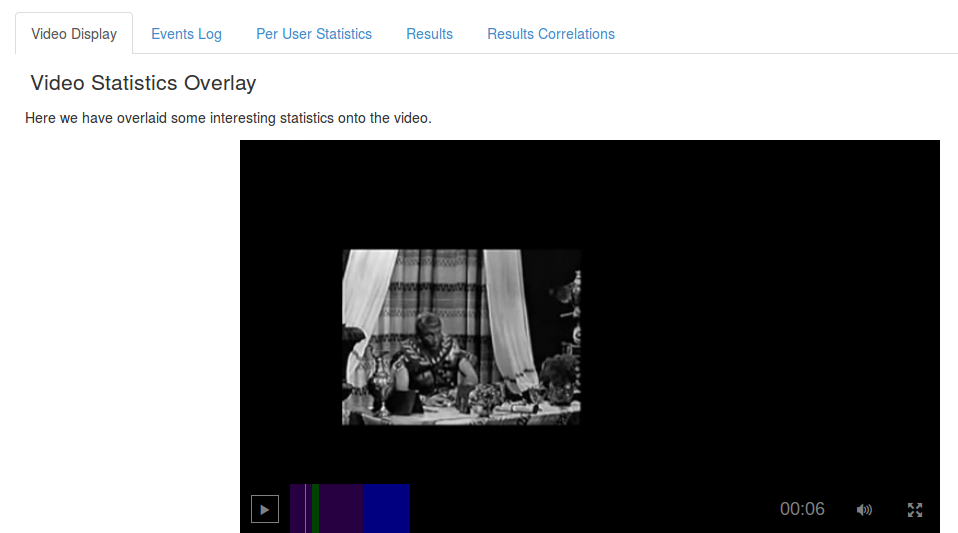
\includegraphics[scale=0.4]{../figures/heatmapDisplay.png}
	\caption{\label{Figure: Heat map display} The heat map has dynamically updated}
\end{figure}

The added feature of displaying the frequencies was also tested. These displayed well and matched the frequencies represented by the colours used. A screen reader could still access the data as it was declared in hidden text.

\subsection{Accessibility}

The example analytics site generally conformed to the WCAG 2.0 standards (see \autoref{table: va conformance}). The non-conformances found were a lack of alternatives for the video and graphs.

The video issues were the same as for the Videogular Questions Example site (see \autoref{Subsection: vqe accessibility}). However the cuepoints were not used. The heatmaps had a textual option that could be displayed which gave additional methods for conveying the information.

Using graphs has created many accessibility issues for visually impaired or cognitively impaired users as the data is not described in text. This would be an important consideration for any developer using our plugins in their own site. As a proof-of-concept our example site purely shows that graphs could be used as a method of automatically producing a visual representation of the data.

\subsection{Deliverable signoff tests}

The tests in table \autoref{table:vgAnalytics Deliverable signoff tests} were presented to the client as the deliverable items for the example analytics tool.

These tests were ran on the analytics tool example using preloaded data so that we had a repeatable set of data that was always valid.

\begin{center}
\begin{longtable}{|L{0.9}|L{0.03}|} 
\caption{\label{table:vgAnalytics Deliverable signoff tests}vgAnalytics Deliverable signoff tests} \\
\hline \textbf{Detail of test} & \rot{\textbf{Pass }}\\ \hline
\endfirsthead
\hline \textbf{Detail of test} & \rot{\textbf{Pass }}\\ \hline \endhead
\multicolumn{2}{c}{Continues on the next page...} \endfoot
\endlastfoot
All events are listed at the top of the events log page, including the type and details of the events & \CheckmarkBold \eoline
The sections that the users have watched are correctly calculated and shown at the bottom & \CheckmarkBold \eoline
Watched video segments are calculated correctly and show how many times all users have viewed a section. & \CheckmarkBold \eoline
The results page shows the user responses. & \CheckmarkBold \eoline
The results page also shows correct answers and whether users rewatched sections. & \CheckmarkBold \eoline
The ``\% watched by correct answers'' and ``Time watched by correct answers'' graphs show two ways you could represent the data in a different way. & \XSolidBrush \eoline
\end{longtable}
\end{center}

Here the final requirement was queried by the customer. The example graphs shown did not have an vertical axis. This was fixed by adding an axis after the customer meeting however during the meeting this did not affect signoff since it was an example of possible graphs that could be created.

\section{Authoring Tool}

The authoring tool is primary deliverable as it is the only item that is designed as a tool and not as a proof of concept example site deliverable. Therefore the primary types of testing are deliverable signoff tests and accessibility testing.

\subsection{Accessibility}
\label{Section:Testing_Authoring_tool_accessibility}

The authoring tool was found to be generally accessible conforming to most of the \gls{WCAG} 2.0 standards (see \autoref{table: authoring tool conformance}). The areas that were lacking were providing textual alternatives and error checking.

There were no alternatives provided for the video. However as this would be used with Synote transcripts could be used from there. In future, support for extra accessibility features such as transcripts, captions or signed versions could be included in the authoring tool.

In creating the questions there is no help provided for error checking. This is because it was decided not to narrow the options available to the users. In the occurrences where errors are identified these are generally highlighted by surrounding the component with a red border. More information on how the system would be used would be required in order to create helpful error messages.

Two keyboard accessibility issues were found, both of which were due to browser bugs. The first was that Google Chrome and Chromium did not allow multiple items to be selected in a \texttt{\textless select multiple\textgreater} element using only the keyboard. During the course of the project, a fix was made to Google Chrome and Chromium which allowed multiple \textit{adjacent} items to be selected with the keyboard \citep{ChromiumMultipleSelectBug}, which is an improvement but still not a complete fix.

The second keyboard accessibility issue was that collapsible section headings caused ``focus loops'' in Mozilla Firefox, where pressing the Tab key from the last button on the heading caused the focus to move back to the heading itself, preventing the user from focussing any content after the heading. This was reported on the Mozilla bug tracker \citep{FirefoxFocusLoopBug} (see \autoref{Chapter:Firefox Bug Report}), where another user pointed out that the HTML causing the bug was invalid. We rewrote the HTML to be valid, which fixed the issue.

Another issue found was in the use of the \texttt{\textless select\textgreater} element as the colour of highlighted options is not editable in the \gls{CSS}. To solve this issue the elements would all need rewriting to take a completely different structure to allow the \gls{CSS} to modify the colours used.

Accessibility in the authoring tool was good but there are improvements that could be made in future including adding support for accessibility features such as subtitles, providing error correction support and rewriting the \texttt{\textless select\textgreater} elements to allow editing of colours.

\subsection{Deliverable signoff tests}

The tests in \autoref{table:Authoring tool Deliverable signoff tests} were presented to the client as the deliverable items for the authoring tool.

\begin{center}
\begin{longtable}{|L{0.9}|L{0.03}|}
\caption{\label{table:Authoring tool Deliverable signoff tests}Authoring tool Deliverable signoff tests} \\
\hline \textbf{Detail of test} & \rot{\textbf{Pass }}\\ \hline
\endfirsthead
\hline \textbf{Detail of test} & \rot{\textbf{Pass }}\\ \hline \endhead
\multicolumn{2}{c}{Continues on the next page...} \endfoot
\endlastfoot
Pressing \keys{Export} will provide you with a \gls{DF} which can be used. & \CheckmarkBold \eoline
Pressing \keys{Preview} will reset the video back to the start, load the questions into the preview, and begin playing & \CheckmarkBold \eoline
All 5 question types are implemented and, as suggested, the Single choice question (with radio buttons) is merged with the Multiple choice question. & \CheckmarkBold \eoline
A question set is able to be added at a specific time. & \CheckmarkBold \eoline
Once a single question has been added the \keys{Preview} button is used to ensure this is shown properly & \CheckmarkBold \eoline
Each question type is tested along with common options and displays as expected. & \CheckmarkBold \eoline
Skipping is tested for one question and works as expected. & \CheckmarkBold \eoline
When checked, the record button sends the poll data to the poll server. & \CheckmarkBold \eoline
A full walkthrough is attempted, all question types are able to be added and previewing, and exporting works & \CheckmarkBold \eoline
\end{longtable}
\end{center}

The pass marks show each test was tested by us and was successful, and also accepted by the client after review of the deliverable report.

\section{Conclusions}

\todo{Comment on the conclusions of the testing.}

